\documentclass[10pt]{article}
\usepackage[letterpaper]{geometry}
\usepackage{listings}
\usepackage{graphicx}
\renewcommand{\figurename}{Imagen}


\title{\textbf{Reporte: Creación de Estructuras con una Calculadora}}
\author{Diego Ruiz Mora | 2202000335}
\date{13-Septiembre-2023}

\begin{document}
	
	\maketitle
	\section{Primera Estructura}
	Para generar la estructura de la \emph{imagen \ref{fig:est1}} tendremos que hacer un pequeño cambio al código donde tendremos que generar solamente un hijo en el código de calculadora y quitar la condición en la que se hacia la petición de una operación a ejecutar. Esto se ve en la \emph{imagen \ref{fig:calculadora}}, que después de la creación del hijo con la instrucción \textbf{idf=fork()}, al hijo le asignamos el nuevo código que en este caso será el de el proceso \emph{suma} como lo hicimos en la tarea, solamente que solo se creará a un hijo en este caso. 
	\\\\
	Por otro lado, para el caso de los procesos hijos es algo parecido, en general notaremos que es la misma modificación para el resto de los códigos, donde buscaremos que cada uno de los procesos tenga un hijo, al que le asignara el código del siguiente proceso, ese siguiente proceso creará un hijo y a su vez le dará el código respectivo del siguiente, así de manera simultanea. 
	\begin{figure}[h!]
		\centering
		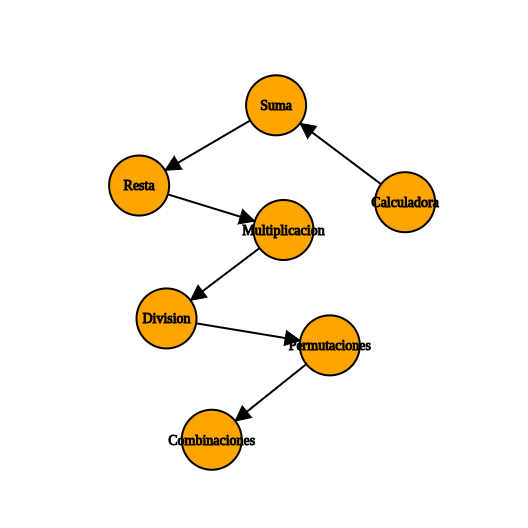
\includegraphics[width=0.5\linewidth]{graph.png}
		\caption{Estructura}
		\label{fig:est1}
	\end{figure}
	\begin{figure}[h!]
		\centering
		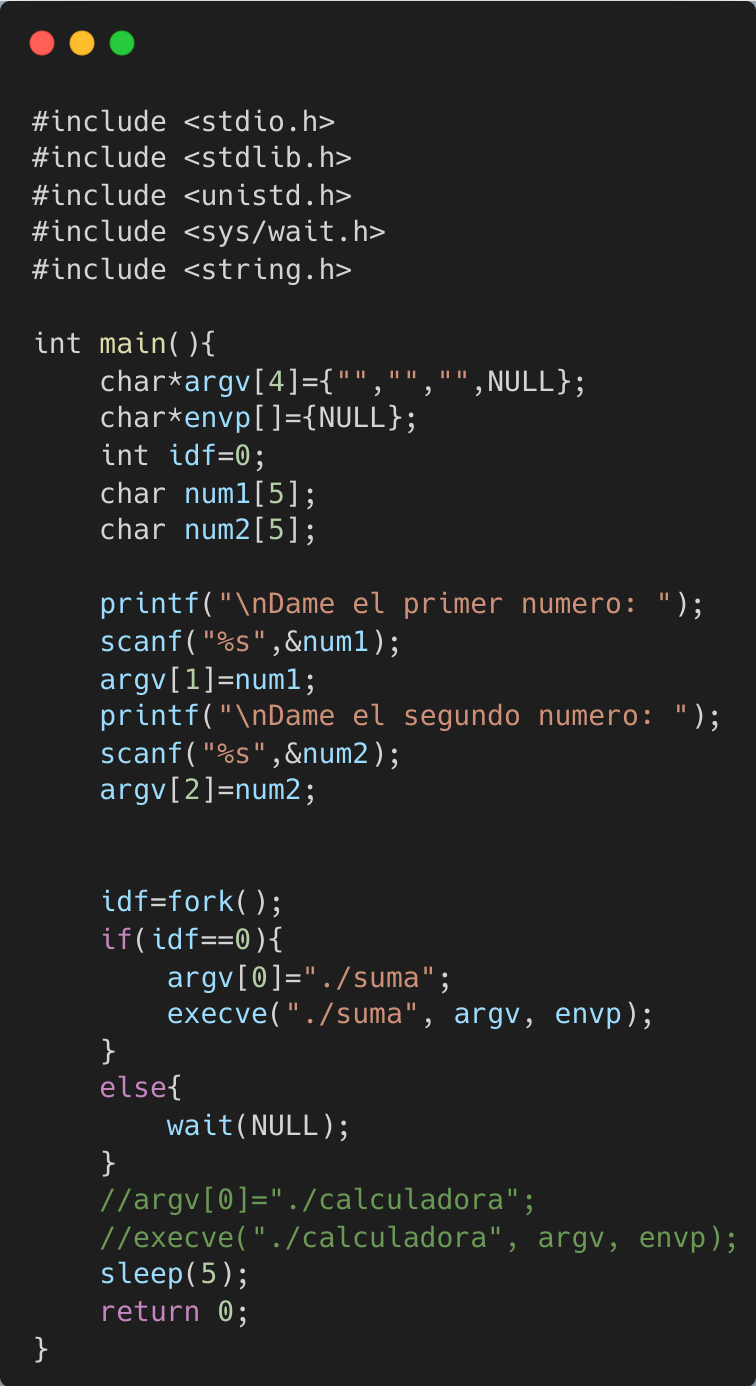
\includegraphics[width=0.4\linewidth]{calculadora.png}
		\caption{Código de calculadora.c}
		\label{fig:calculadora}
	\end{figure}
	\newpage
	Para ver de manera más fiel de lo que hablamos, tendremos que recurrir a la \emph{imagen \ref{fig:suma}}, donde veremos el código respectivo para la \emph{suma} y como es que creamos un hijo y después le asignamos a este hijo el código de la siguiente operación. 
	\\\\
	Y como bien dijimos esto se repetirá hasta que se llegue al último proceso que es \emph{combinaciones} que es el que no se verá modificado en su código. También es importante denotar que en los demás códigos incorporemos una instrucción \textbf{wait(NULL)} que nos permitirá esperar a que los procesos hijos dejen de ejecutar para que los procesos padres terminen. Esto nos permitirá visualizar el árbol de procesos. 
	\begin{figure}[h!]
		\centering
		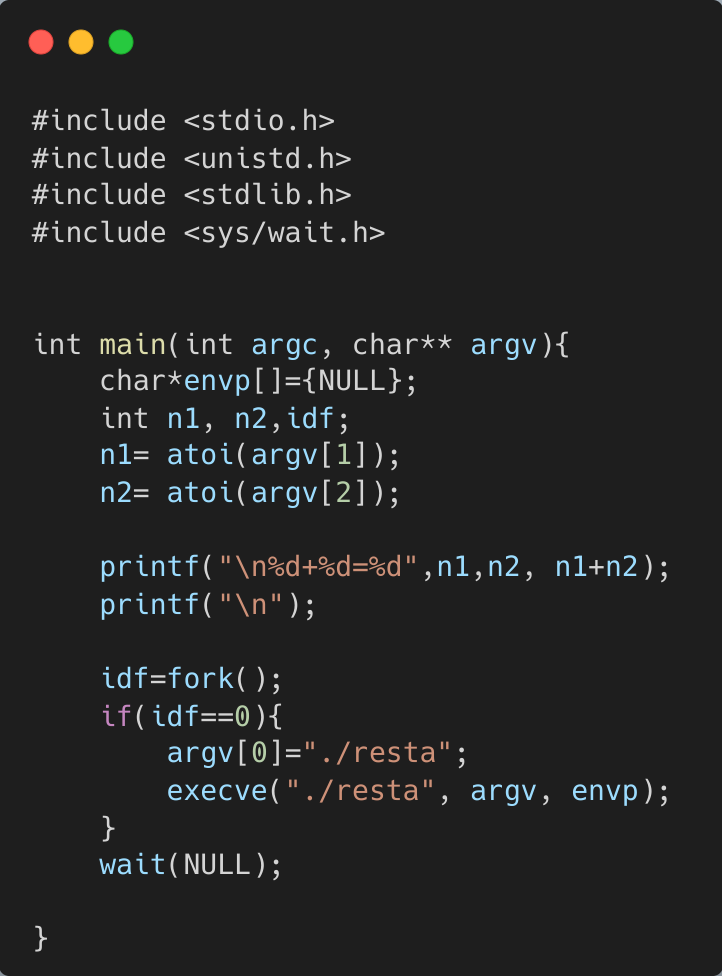
\includegraphics[width=0.4\linewidth]{suma.png}
		\caption{Código de suma.c}
		\label{fig:suma}
	\end{figure}
	\\\\
	Veremos en la \emph{imagen \ref{fig:pruebae1}} que es correcta esta forma de realizar el código ya que la estructura generada es la deseada, donde cada uno de los procesos tiene un hijo que es el siguiente proceso a ejecutar. De igual forma al ver el código ejecutado notaremos que los valores que pasan son los mismo, ya que esto no se modificó, aunque si se podría lograr modificando el vector de argumentos en cada proceso antes de asignar el código al siguiente hijo. 
	\begin{figure}[h!]
		\centering
		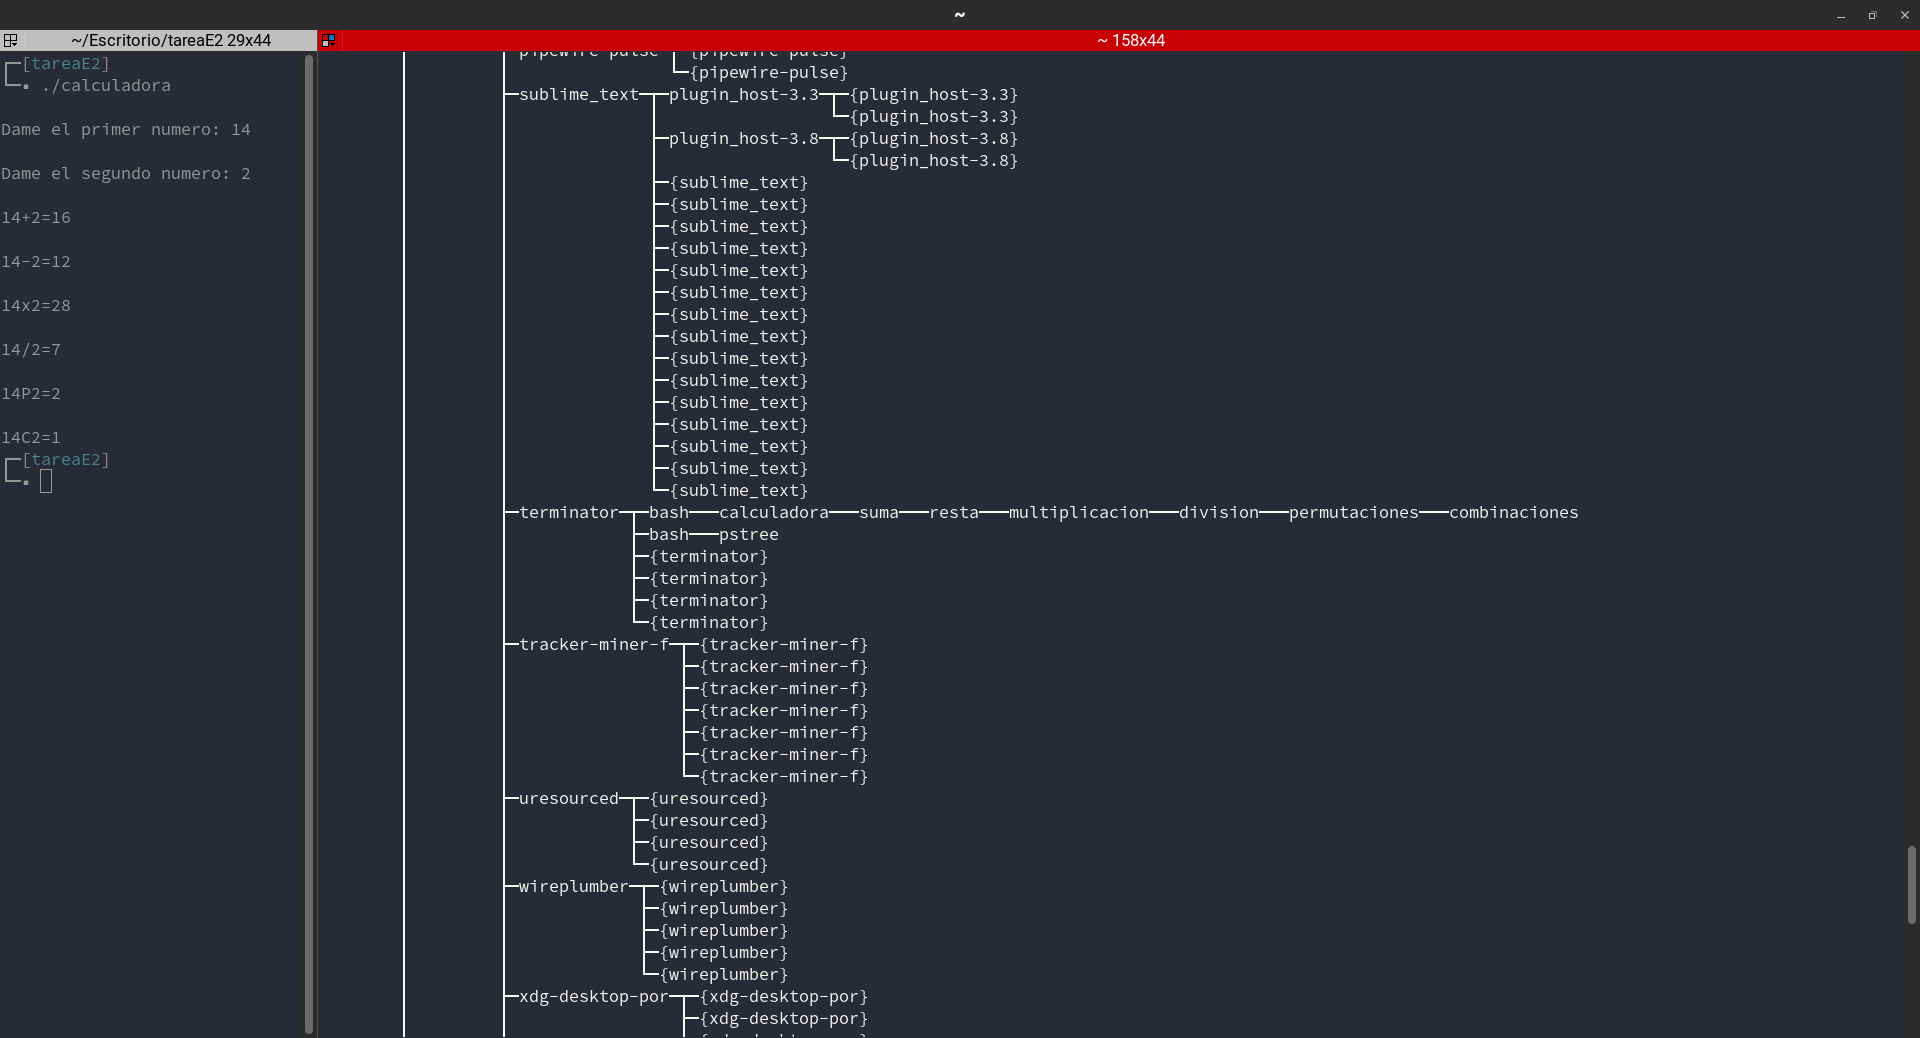
\includegraphics[width=\linewidth]{pruebaE1}
		\caption{Estructura generada}
		\label{fig:pruebae1}
	\end{figure}
	\newpage
	
	\section{Segunda Estructura}
	Para realizar la siguiente estructura mostrada en \emph{imagen  \ref{fig:est2}} modificaremos solamente tres códigos que serán: \emph{calculadora.c, division.c y resta.c}. 
	A los dos últimos solamente haremos un hijo como en el caso de la estructura pasada y en caso de \emph{calculadora} crearemos cuatro hijos. 
	\begin{figure}[h!]
		\centering
		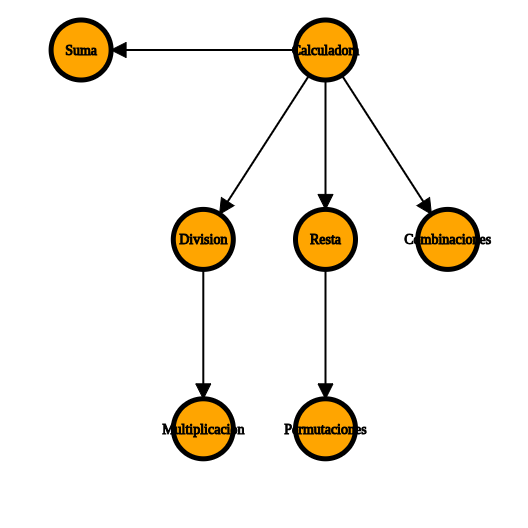
\includegraphics[width=0.5\linewidth]{graph2.png}
		\caption{Estructura}
		\label{fig:est2}
	\end{figure}
	\\
	Primero revisaremos el código respectivo a \emph{calculadora} donde, como bien lo mencionamos tenemos la creación de cuatro hijos para los procesos que son el primer nivel del árbol. Cada uno tiene un \textbf{idf} distinto, ya que lo que buscamos es identificar cada uno de ellos, ya que al asignarle el código tendremos que ser muy específicos para no incurrir en duplicados. 
	\\
	Es más sencillo hacerlo de esta manera, ya que si reutilizamos el identificador del proceso se vuelve una tarea complicada de hacer.
	\\\\
	Por otro lado, notaremos que no incorporamos una llamada a sistema \textbf{wait(NULL)} que nos ayudaría a que este proceso no termine hasta que los hijos terminen, esto nos permitiría visualizar la estructura y que no tengamos conflictos de que se terminen unos antes que otros, pero curiosamente, funciona mejor sin esta instrucción, entonces la omitimos en este caso.
	\\\\
	Después de ello tendremos que modificar los procesos que generan otros hijos, que en este caso son \emph{division y resta} para lo cuál solamente tenemos que hacer un hijo al final del código, que es de suma importancia para que no se repita el código o impresiones de datos. 
	\begin{figure}[h!]
		\centering
		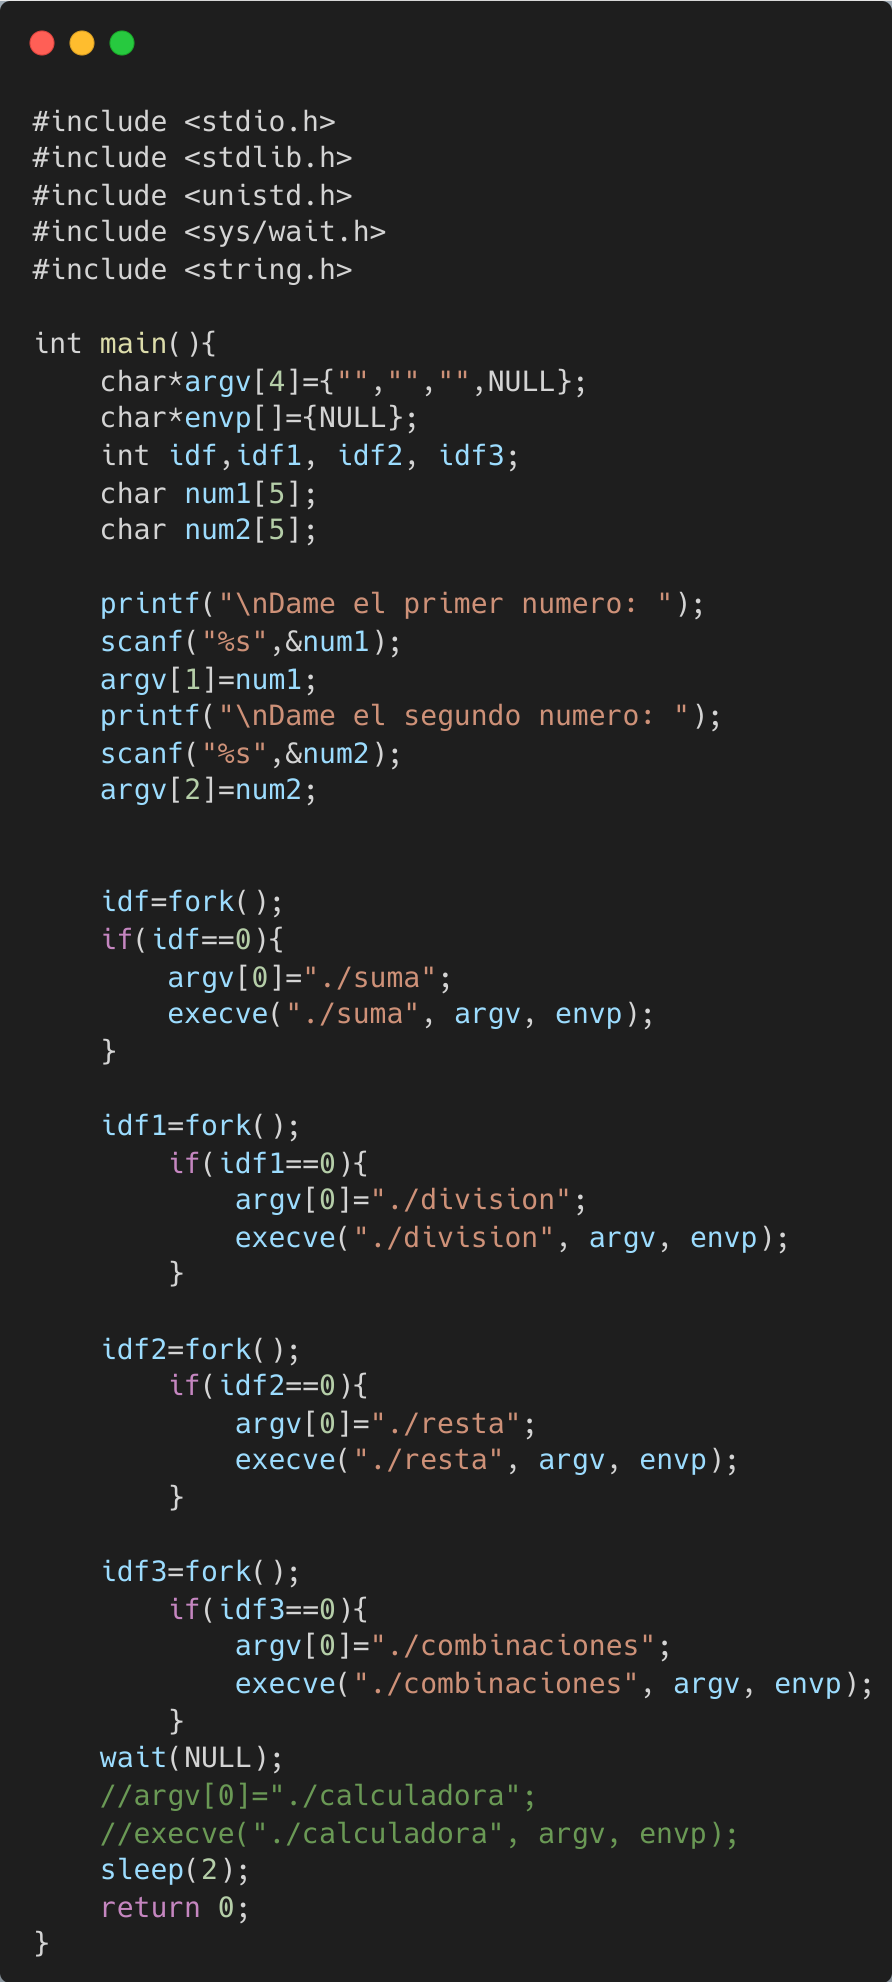
\includegraphics[width=0.5\linewidth]{calculadora2.png}
		\caption{Código calculadora.c}
		\label{fig:calculadora2}
	\end{figure}
	\newpage
	Como vemos en la \emph{imagen \ref{fig:division}} mediante la llamada a sistema \textbf{fork()} creamos un proceso hijo en el proceso \emph{division} y a ese hijo le asignamos el código de \emph{multiplicacion}, por último hacemos lo mismo que antes, utilizar la instrucción \textbf{wait()} para que este proceso termine después que el proceso hijo.
	\begin{figure}[h!]
		\centering
		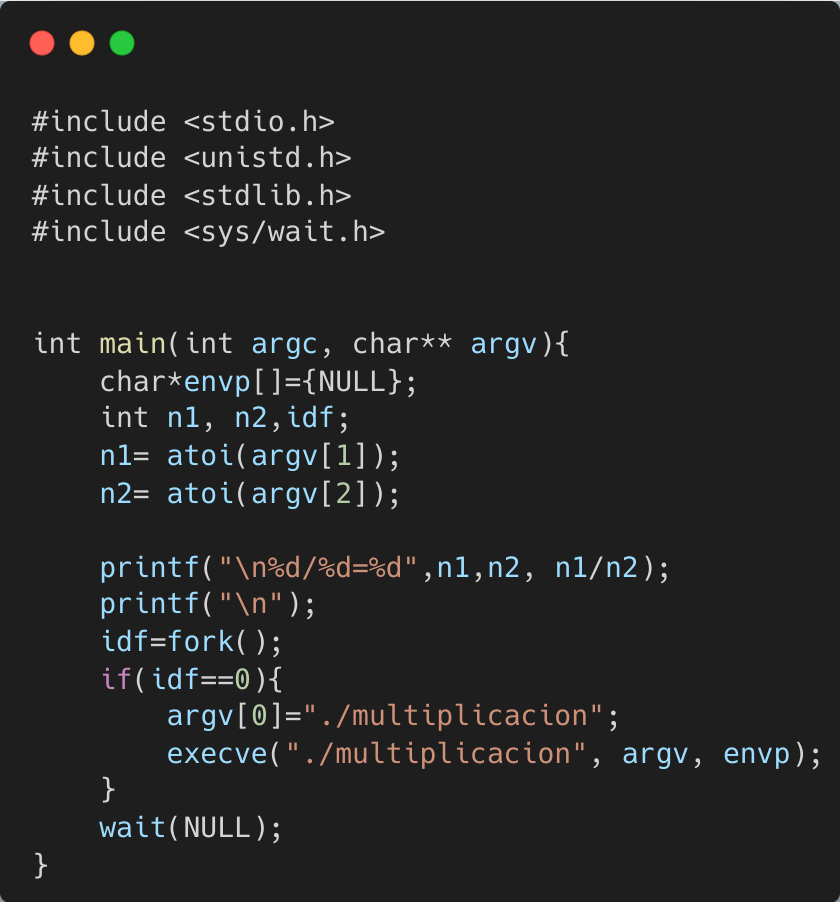
\includegraphics[width=0.5\linewidth]{division.png}
		\caption{Código division.c}
		\label{fig:division}
	\end{figure}
	\\\\
	Lo mismo sucederá  en el caso del proceso \emph{resta} que tendrá como hijo al proceso \emph{permutaciones}, lograrlo es básicamente hacer lo mismo, crear un hijo y asignarle el código del proceso correspondiente.  Y que no se nos olvidé colocar la instrucción que espera a que el proceso hijo termine. 
	\\\\
	Por otro lado, para el resto de procesos que son solamente hijos, agregamos una instrucción \textbf{sleep(2)} al final, esto con el fin de visualizar la estructura y que los procesos que no tienen hijos no terminen tan pronto. Realmente es el único cambio que se realiza en estos procesos, ya que fuera de ello no necesita más tratamiento. 
	\\\\
	Como veremos en la \emph{imagen \ref{fig:pruebae2}} al ejecutar la \emph{calculadora} verificamos que la estructura generada es igual a la deseada, donde los hijos de medio tendrán a sus dos respectivos hijos de hecho al notar como es que entrega resultados el programa, primero se dan los resultados del primer nivel del árbol y luego se dan los resultados del segundo nivel. 
	\\\\
	De esta manera podemos llegar a las estructuras deseadas, desde mi punto de vista es más sencillo realizarlo así ya que los hijos pueden tener un código propio, esto facilita ya que no necesitamos crear toda la estructura desde \emph{calculadora}, al contrario, podemos dividir la creación de procesos para que cada proceso cree el hijo o hijos que requiera, incluso creo que es una buena práctica realizarlo así, es parecido a la POO.
	\begin{figure}[h!]
		\centering
		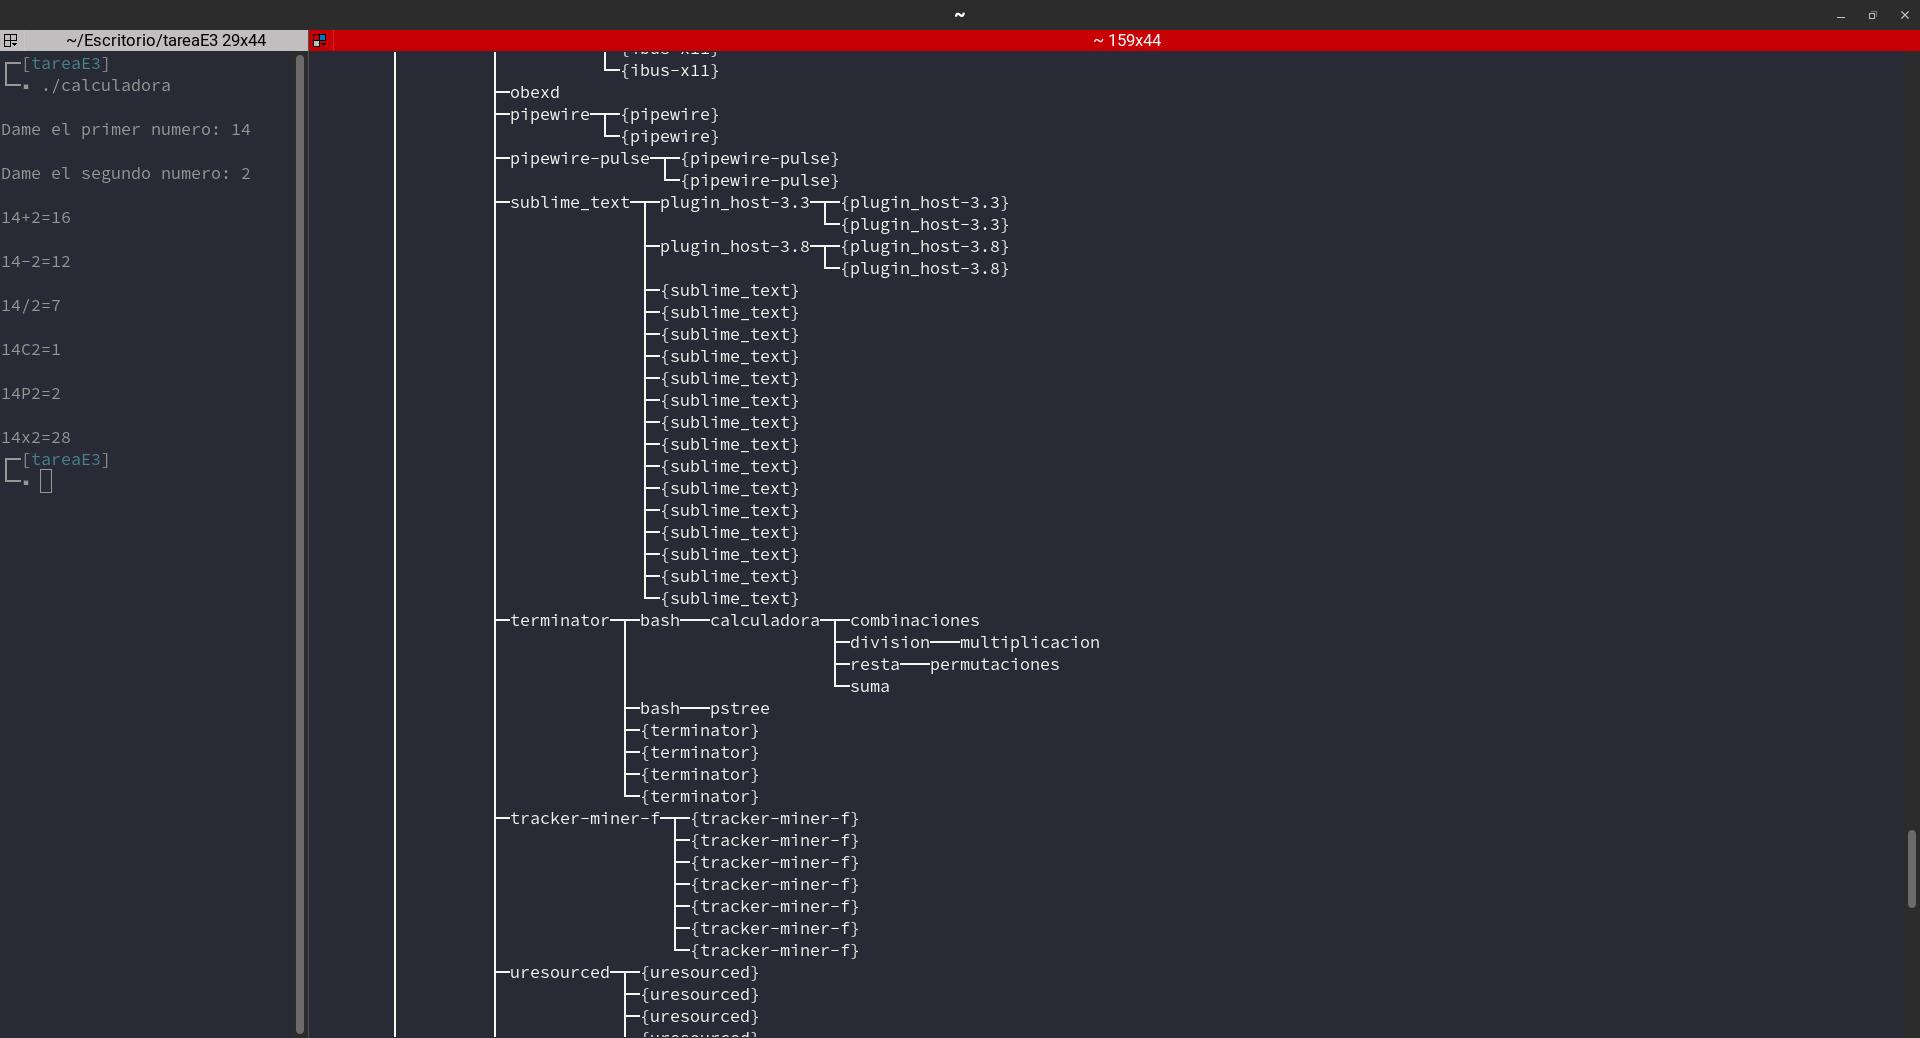
\includegraphics[width=\linewidth]{pruebaE2.png}
		\caption{Estructura generada}
		\label{fig:pruebae2}
	\end{figure}

	
	
\end{document}